% 基本群：平面去掉原点，alpha 绕洞一周（生成元），beta 零伦
\documentclass[border=4pt]{standalone}
\usepackage{tikz}
\usetikzlibrary{arrows.meta}
\usepackage{amsmath,amssymb}
\definecolor{fillA}{rgb}{0.45,0.45,0.45}
\definecolor{fillB}{rgb}{0.72,0.72,0.72}
\begin{document}
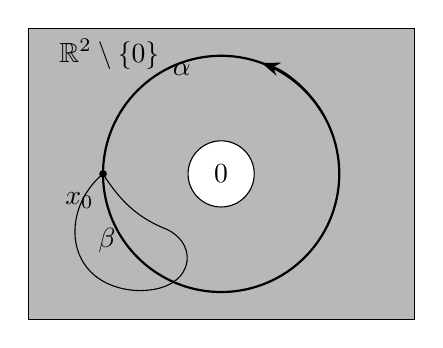
\begin{tikzpicture}[>=Stealth, line cap=round]
% 平面区域（挖去原点：even odd rule 得到透明洞）
\fill[fillB, even odd rule] (0.35,0.35) rectangle (5.25,4.05) (2.8,2.2) circle (0.42);
\draw (0.35,0.35) rectangle (5.25,4.05);
\draw (2.8,2.2) circle (0.42);
\node at (2.8,2.2) {$0$};
\node[anchor=west] at (0.62,3.72) {$\mathbb R^2\setminus\{0\}$};
% 生成元 alpha：绕洞一周
\draw[thick] (1.3,2.2) arc (180:540:1.5);
\draw[thick, ->] (4.099,2.95) arc (30:70:1.5);
\node at (2.3,3.52) {$\alpha$};
% 零伦环路 beta：不绕洞
\draw (1.3,2.2) .. controls (0.75,1.75) and (0.8,0.8) .. (1.7,0.72)
  .. controls (2.45,0.68) and (2.55,1.3) .. (2.1,1.5)
  .. controls (1.8,1.62) and (1.55,1.8) .. (1.3,2.2);
\node at (1.35,1.35) {$\beta$};
% 基点 x0
\fill (1.3,2.2) circle (1.4pt);
\node at (1.0,1.86) {$x_0$};
\end{tikzpicture}
\end{document}
